En los últimos años, el análisis de datos ha adquirido un papel fundamental dentro del fútbol profesional, dando lugar al desarrollo del denominado \textit{Sports Analytics}. Esta disciplina combina técnicas de estadística, inteligencia artificial y aprendizaje automático con el objetivo de extraer conocimiento útil a partir de grandes volúmenes de datos deportivos. Según Bassek et al. \cite{bassek_integrated_2025}, el creciente acceso a datos de eventos, posicionamiento y vídeo ha impulsado el desarrollo de nuevas metodologías para el análisis del rendimiento de jugadores y equipos, así como para la predicción de resultados y la evaluación táctica.

No obstante, los propios autores señalan que uno de los principales desafíos actuales consiste en la disponibilidad de conjuntos de datos públicos, completos y estructurados que permitan desarrollar modelos reproducibles y comparar distintas metodologías de investigación \cite{bassek_integrated_2025}. Esta limitación ha motivado la creación de nuevas bases de datos abiertas que faciliten el avance de la investigación en este ámbito.

La aplicación de técnicas de aprendizaje automático e inteligencia artificial al fútbol también ha experimentado un crecimiento significativo durante los últimos años. Diversos estudios muestran que los modelos predictivos y de clasificación permiten identificar patrones complejos y apoyar tareas como la predicción de resultados, la evaluación del rendimiento y la toma de decisiones deportivas \cite{fotache_machine_2026, rahman_artificial_2026, liu_application_2025}. Estos avances han convertido estas técnicas en herramientas de apoyo cada vez más relevantes para analistas, entrenadores y departamentos de \textit{scouting}.

Paralelamente, el crecimiento del volumen de información disponible ha incrementado la importancia de las técnicas de \textit{business intelligence}. Según el estudio \textit{Development of a Dashboard for Big Data Analysis}, los cuadros de mando permiten transformar grandes cantidades de datos en información fácilmente interpretable mediante indicadores clave (\textit{KPI}) y representaciones gráficas, facilitando la detección de tendencias y la toma de decisiones \cite{marcelo_business_2023}. Esta filosofía constituye uno de los pilares de la aplicación desarrollada en este trabajo, donde la información obtenida mediante diferentes técnicas de análisis se presenta a través de \textit{dashboards} interactivos orientados a facilitar su interpretación.

El uso de estas metodologías ya no se limita al ámbito académico. Tal y como recoge la investigación centrada en el Brentford FC \cite{kane_how_2026}, los clubes profesionales pueden utilizar modelos analíticos para optimizar procesos relacionados con el análisis del rendimiento, la planificación deportiva, la detección de talento y la política de fichajes. Este cambio refleja la importancia que ha adquirido la analítica de datos como herramienta de apoyo dentro del fútbol moderno.

Por otra parte, las aplicaciones deportivas constituyen un medio cada vez más relevante para acercar información y servicios relacionados con el deporte al usuario final. Chembakottu et al. \cite{chembakottu_large-scale_2023} analizaron más de 2.000 aplicaciones deportivas disponibles en Google Play con el objetivo de estudiar sus principales características y la percepción de los usuarios a partir de sus reseñas. El estudio pone de manifiesto la diversidad de funcionalidades presentes en este tipo de aplicaciones y la utilidad del análisis de datos para identificar necesidades de los usuarios y posibles mejoras. En este contexto, existe interés en desarrollar soluciones que, además de facilitar la consulta de información deportiva, incorporen herramientas de análisis capaces de aportar un mayor valor al usuario.

Aunque la inteligencia artificial y el aprendizaje automático han ganado presencia en el análisis futbolístico, una parte relevante de la investigación sobre predicción de resultados se ha orientado hacia su aplicación en mercados de apuestas deportivas. Algunos trabajos estudian si los modelos de \textit{machine learning} pueden superar las predicciones de las casas de apuestas o generar estrategias rentables en mercados concretos, como el resultado del partido o la probabilidad de que ambos equipos marquen \cite{DACOSTA2022895, HUBACEK2019783}. Esta línea de investigación demuestra el potencial predictivo de estas técnicas, pero también evidencia que muchas aplicaciones se centran más en el valor económico de la predicción que en proporcionar herramientas comprensibles para el análisis deportivo.

\section{Técnicas de aprendizaje automático y simulación}

El aprendizaje automático permite identificar patrones y extraer conocimiento a partir de grandes volúmenes de datos. En el fútbol profesional, su utilización ha crecido notablemente en los últimos años, tanto en tareas relacionadas con el análisis del rendimiento de jugadores y equipos como en la predicción de resultados. Una revisión de 172 estudios publicados entre 2019 y 2024 muestra un predominio de las técnicas de aprendizaje supervisado, \textit{deep learning} y modelos híbridos, destacando el uso de algoritmos como los árboles de decisión, \textit{random forest}, \textit{XGBoost} y las redes neuronales \cite{moya_machine_2025}.

Dentro de este contexto, en el presente trabajo se emplean técnicas pertenecientes a distintas familias. Por un lado, se utilizan métodos de aprendizaje no supervisado para descubrir agrupaciones naturales entre jugadores con características estadísticas similares. Por otro lado, se aplican modelos de aprendizaje supervisado para estimar resultados a partir de datos históricos previamente etiquetados. Además, se incorporan métodos de simulación probabilística que permiten proyectar distintos escenarios de una temporada completa. Esta combinación permite abordar el análisis futbolístico desde varias perspectivas: la comparación de jugadores, la predicción de partidos y la estimación de posibles desenlaces competitivos.

\subsection{\textit{K-means}}

El algoritmo \textit{K-means} se ha utilizado en este proyecto para agrupar jugadores según sus características estadísticas y obtener perfiles similares dentro de la base de datos. Al tratarse de una técnica de aprendizaje no supervisado, no necesita una variable objetivo previamente definida, sino que busca organizar los datos en distintos \textit{clusters} a partir de la similitud entre las observaciones.

Esta técnica resulta especialmente útil en el ámbito futbolístico, ya que permite comparar jugadores más allá de métricas individuales aisladas. En lugar de analizar únicamente goles, asistencias o minutos disputados, el agrupamiento permite identificar futbolistas con comportamientos estadísticos parecidos, lo que puede servir como apoyo para tareas de análisis de rendimiento, comparación de perfiles o búsqueda de jugadores similares. En esta línea, Azzami et al. \cite{azzami_clustering_2025} aplicaron \textit{K-means} sobre datos de 17.947 jugadores, considerando variables de rendimiento, posición, características físicas y valor de mercado, y obtuvieron distintos perfiles que evidencian la utilidad de esta técnica en el análisis de futbolistas.

\subsection{\textit{Random forest}}

Para la predicción de partidos se ha considerado el uso de \textit{random forest}, un algoritmo de aprendizaje supervisado basado en la combinación de múltiples árboles de decisión. Cada árbol se entrena con una parte de los datos y genera una predicción individual, que posteriormente se combina con el resto para obtener el resultado final. Esta estrategia permite mejorar la estabilidad del modelo y reducir el riesgo de sobreajuste respecto al uso de un único árbol de decisión \cite{pugsee_football_2019}.

Su aplicación resulta adecuada en problemas futbolísticos porque el resultado de un partido depende de múltiples factores que no siempre presentan relaciones lineales simples. Variables como la forma reciente, la diferencia de goles, los resultados previos, el rendimiento local o visitante y la posición clasificatoria pueden interactuar de forma compleja. Por ello, este tipo de modelos se ha utilizado en estudios de predicción de resultados, como el de Pugsee y Pattawong \cite{pugsee_football_2019}, centrado en partidos de la Premier League. También se ha empleado en otros análisis deportivos, como el estudio de Van Arem et al. \cite{arem_forecasting_2025}, donde \textit{random forest} fue seleccionado como el modelo más adecuado para predecir la evolución futura del rendimiento y del valor de jugadores profesionales.

\subsection{Simulación de Monte Carlo}

Junto a los modelos de aprendizaje automático, el proyecto incorpora la simulación de Monte Carlo como método probabilístico para analizar posibles desenlaces de una temporada. A diferencia de los algoritmos anteriores, esta técnica no aprende directamente patrones a partir de los datos, sino que genera un gran número de escenarios aleatorios basados en probabilidades previamente calculadas. De esta forma, permite estimar la frecuencia con la que se producen determinados resultados tras repetir muchas veces una misma situación.

En el contexto del fútbol, este enfoque es útil porque una competición no depende únicamente de un partido aislado, sino de la acumulación de muchos encuentros y de la interacción entre los resultados de todos los equipos. Por ello, la simulación permite estimar probabilidades asociadas a distintas posiciones finales, como el título de liga, la clasificación europea, la permanencia o el descenso. Stock et al. \cite{stock_physics-based_2022} emplean este tipo de simulaciones para predecir la evolución de diferentes ligas de fútbol, mientras que Tűű-Szabó y Kóczy \cite{tuu-szabo_monte_2026} combinan modelos probabilísticos de resultados con simulaciones de Monte Carlo para analizar el impacto del calendario sobre la clasificación final.
\section{Aplicaciones similares} 

Para analizar qué ventajas puede aportar este proyecto frente a otras soluciones existentes, se realiza una comparación con tres aplicaciones representativas del mercado: \textit{BeSoccer} \cite{besoccer}, \textit{SofaScore} \cite{noauthor_futbol_nodate} y la aplicación oficial de LaLiga \cite{noauthor_pagina_2026}. Estas han sido seleccionadas por su popularidad, su amplio número de usuarios y por representar distintos enfoques dentro de las aplicaciones de seguimiento y análisis futbolístico.

Aunque existen otras alternativas populares, como \textit{OneFootball} o \textit{Flashscore}, la mayoría de ellas siguen un modelo funcional similar, centrado principalmente en resultados, calendarios, clasificaciones, noticias y estadísticas básicas. Por este motivo, el análisis se centra en las tres aplicaciones mencionadas, ya que permiten cubrir las funcionalidades estándar del sector y sirven como referencia para destacar el valor añadido de la propuesta desarrollada, especialmente en lo relativo al análisis avanzado, la predicción de resultados y la aplicación de técnicas de minería de datos.

\begin{itemize}
    \item Aplicación oficial de LaLiga: se trata de la aplicación desarrollada por la propia organización de LaLiga. Su funcionalidad principal se centra en la consulta de resultados, resúmenes de partidos, noticias, calendarios y clasificaciones. Aunque cuenta con información oficial de la competición, el nivel de análisis estadístico ofrecido es limitado y no incorpora funcionalidades avanzadas basadas en inteligencia artificial o aprendizaje automático orientadas al usuario final.

    Su principal fortaleza reside en la fiabilidad y oficialidad de los datos relacionados con LaLiga y LaLiga Hypermotion. No obstante, en otras competiciones su alcance se reduce principalmente a la consulta de resultados. Como se observa en la Figura~\ref{fig:laliga}, la aplicación ofrece información útil para el seguimiento básico de la competición, pero con una profundidad analítica reducida, especialmente si se tiene en cuenta la disponibilidad actual de métricas avanzadas y la colaboración de LaLiga con empresas especializadas en datos, como Opta.
\end{itemize}

\begin{figure}[H]
\centering
  \begin{subfigure}[b]{0.4\textwidth}
    \centering
    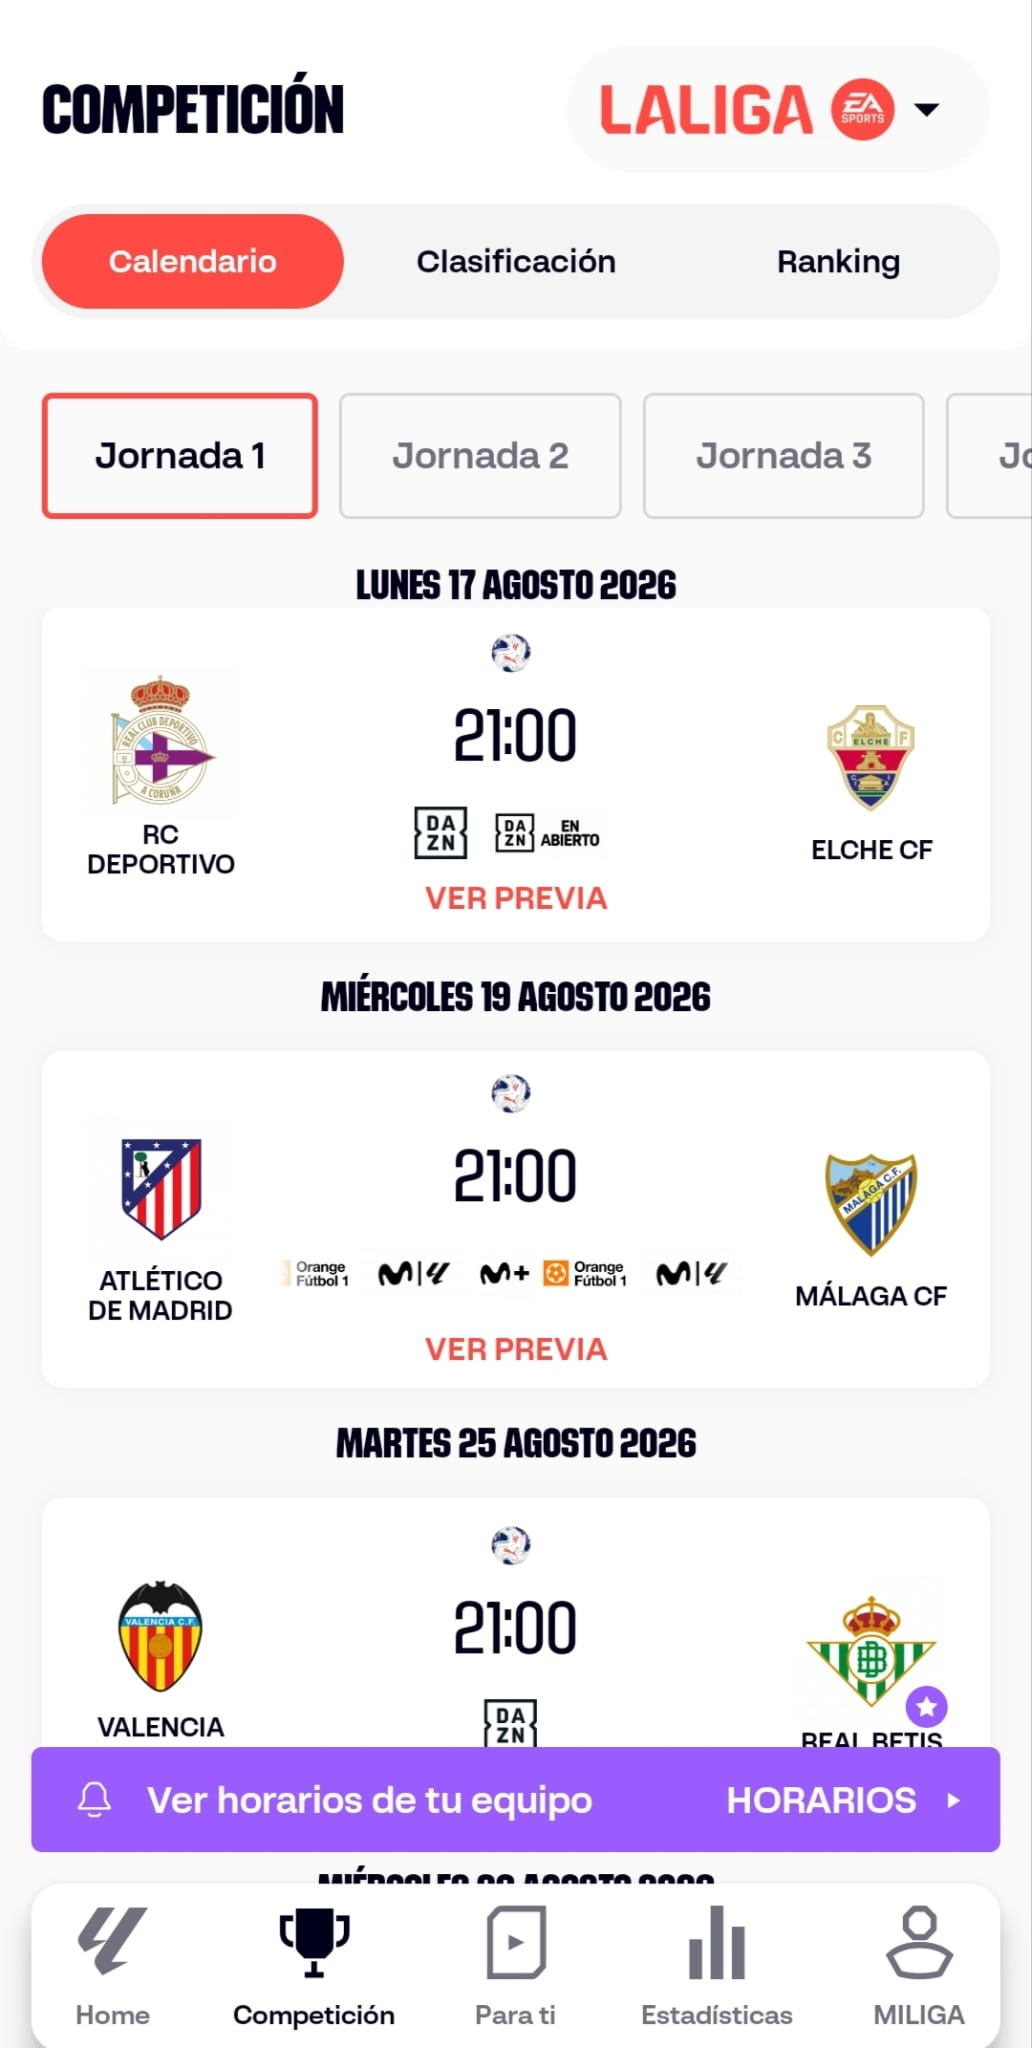
\includegraphics[width=0.5\linewidth]{figures/app_lalila.jpeg}
    \caption{Pantalla de resultados}
    \label{fig:laliga_resultados}
  \end{subfigure}
  \hspace{0.5cm}
  \begin{subfigure}[b]{0.4\textwidth}
    \centering
    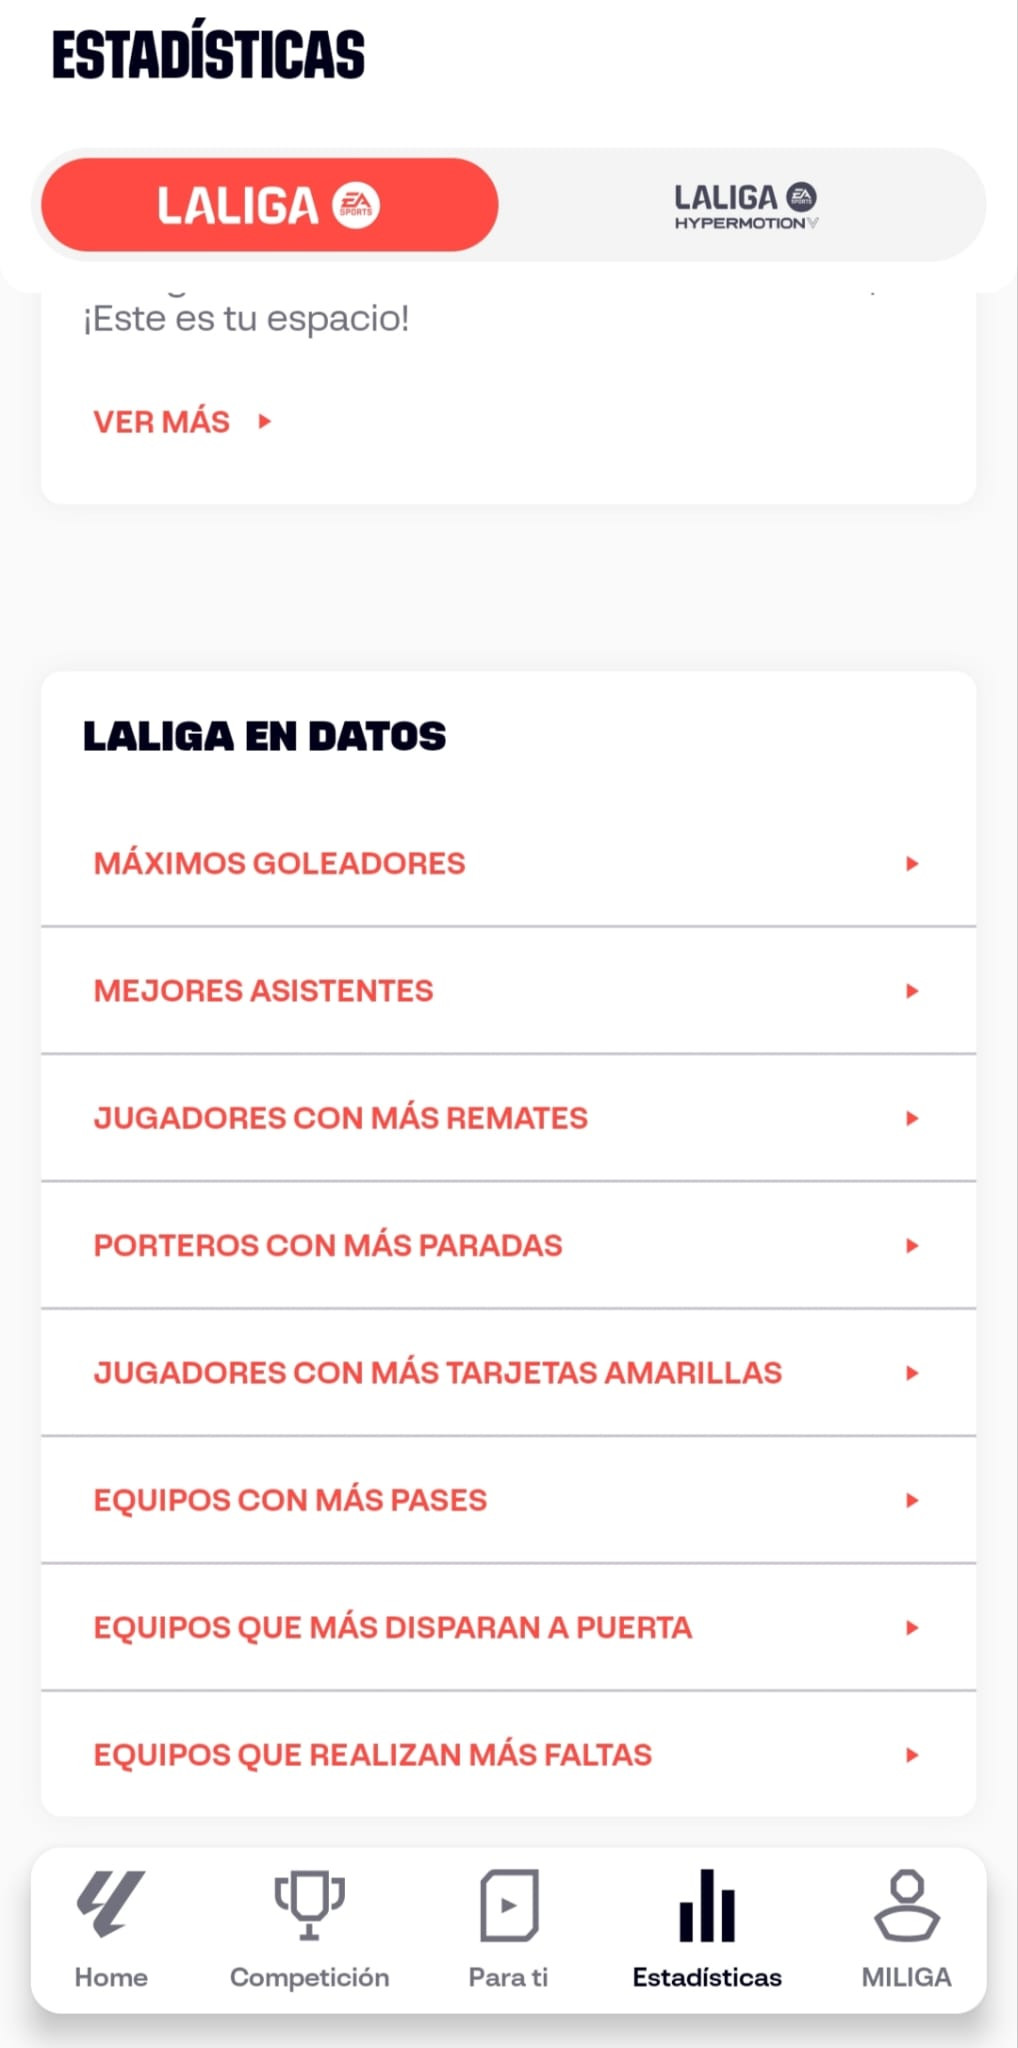
\includegraphics[width=0.5\linewidth]{figures/app_laliga_stats.jpeg}
    \caption{Estadísticas mostradas}
    \label{fig:laliga_stats}
  \end{subfigure}
  \caption{Aplicación oficial de LaLiga}
  \label{fig:laliga}
\end{figure}

\begin{itemize}
    \item BeSoccer: es una aplicación con una cobertura muy amplia, ya que incluye información sobre numerosas ligas y competiciones de fútbol a nivel mundial. Ofrece calendario, clasificaciones, noticias, fichajes, estadísticas de equipos y datos básicos de jugadores. En el apartado de partidos, incorpora información previa como probabilidades, rankings ELO y algunos gráficos comparativos entre equipos, tal y como se muestra en la Figura~\ref{fig:besoccer}.

    Sin embargo, el análisis individual de jugadores es más limitado, ya que se centra principalmente en estadísticas tradicionales como goles, asistencias, tarjetas o partidos disputados. Aunque incluye algunos elementos visuales, como radares de atributos, no siempre se muestra con claridad la base estadística utilizada para construir dichos indicadores. En cuanto al análisis de temporada, destaca la presencia de clasificaciones con probabilidades por rango basadas en simulaciones de Monte Carlo y rankings estadísticos básicos. Por tanto, BeSoccer ofrece una cobertura muy completa, pero su análisis avanzado queda centrado principalmente en determinadas secciones y no se presenta como una herramienta integral de minería de datos.
\end{itemize}

\begin{figure}[H]
\centering
  \begin{subfigure}[b]{0.4\textwidth}
    \centering
    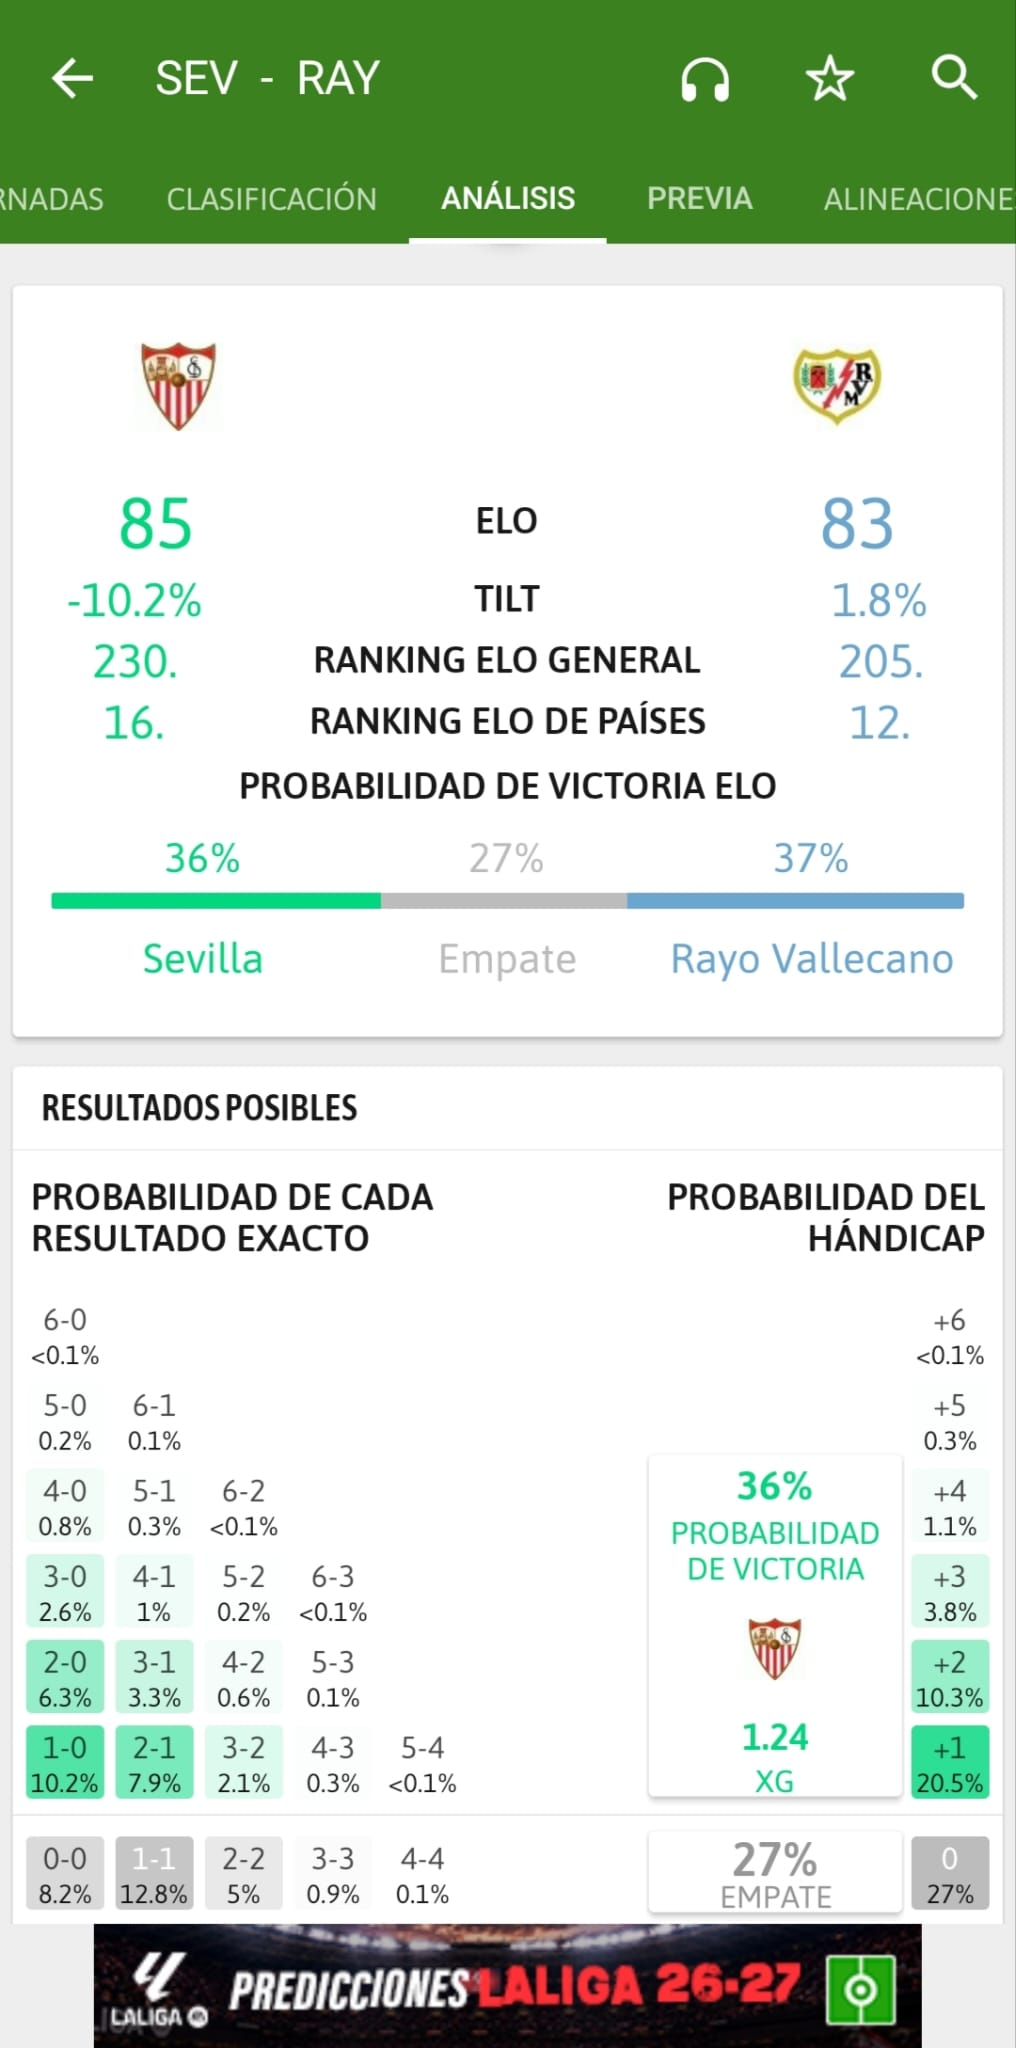
\includegraphics[width=0.5\linewidth]{figures/app_besoccer_prob.jpeg}
    \caption{Pantalla de probabilidades}
    \label{fig:besoccer_prob}
  \end{subfigure}
  \caption{BeSoccer}
  \label{fig:besoccer}
\end{figure}

\begin{itemize}
    \item SofaScore: es probablemente la aplicación más avanzada de las tres en cuanto a volumen de información y nivel estadístico. Su alcance no se limita al fútbol, sino que abarca numerosos deportes y competiciones. En el caso del fútbol, ofrece estadísticas detalladas de partidos, mapas de calor, valoraciones individuales de jugadores, datos de rendimiento y comparativas avanzadas.

    Uno de sus elementos más destacados es el sistema de valoración individual de jugadores, que permite evaluar el rendimiento de cada futbolista en un partido concreto. Como se aprecia en la Figura~\ref{fig:sofascore}, SofaScore ofrece una mayor profundidad estadística que las aplicaciones anteriores. No obstante, parte de sus funcionalidades más avanzadas, especialmente aquellas relacionadas con inteligencia artificial, se encuentran asociadas a servicios de pago. Además, una parte importante de sus análisis previos está orientada al contexto de las apuestas deportivas, lo que puede alejarse del enfoque puramente analítico y académico que persigue este proyecto. A pesar de ello, SofaScore constituye una referencia clara en cuanto a visualización de datos deportivos y profundidad estadística.
\end{itemize}

\begin{figure}[H]
\centering
  \begin{subfigure}[b]{0.4\textwidth}
    \centering
    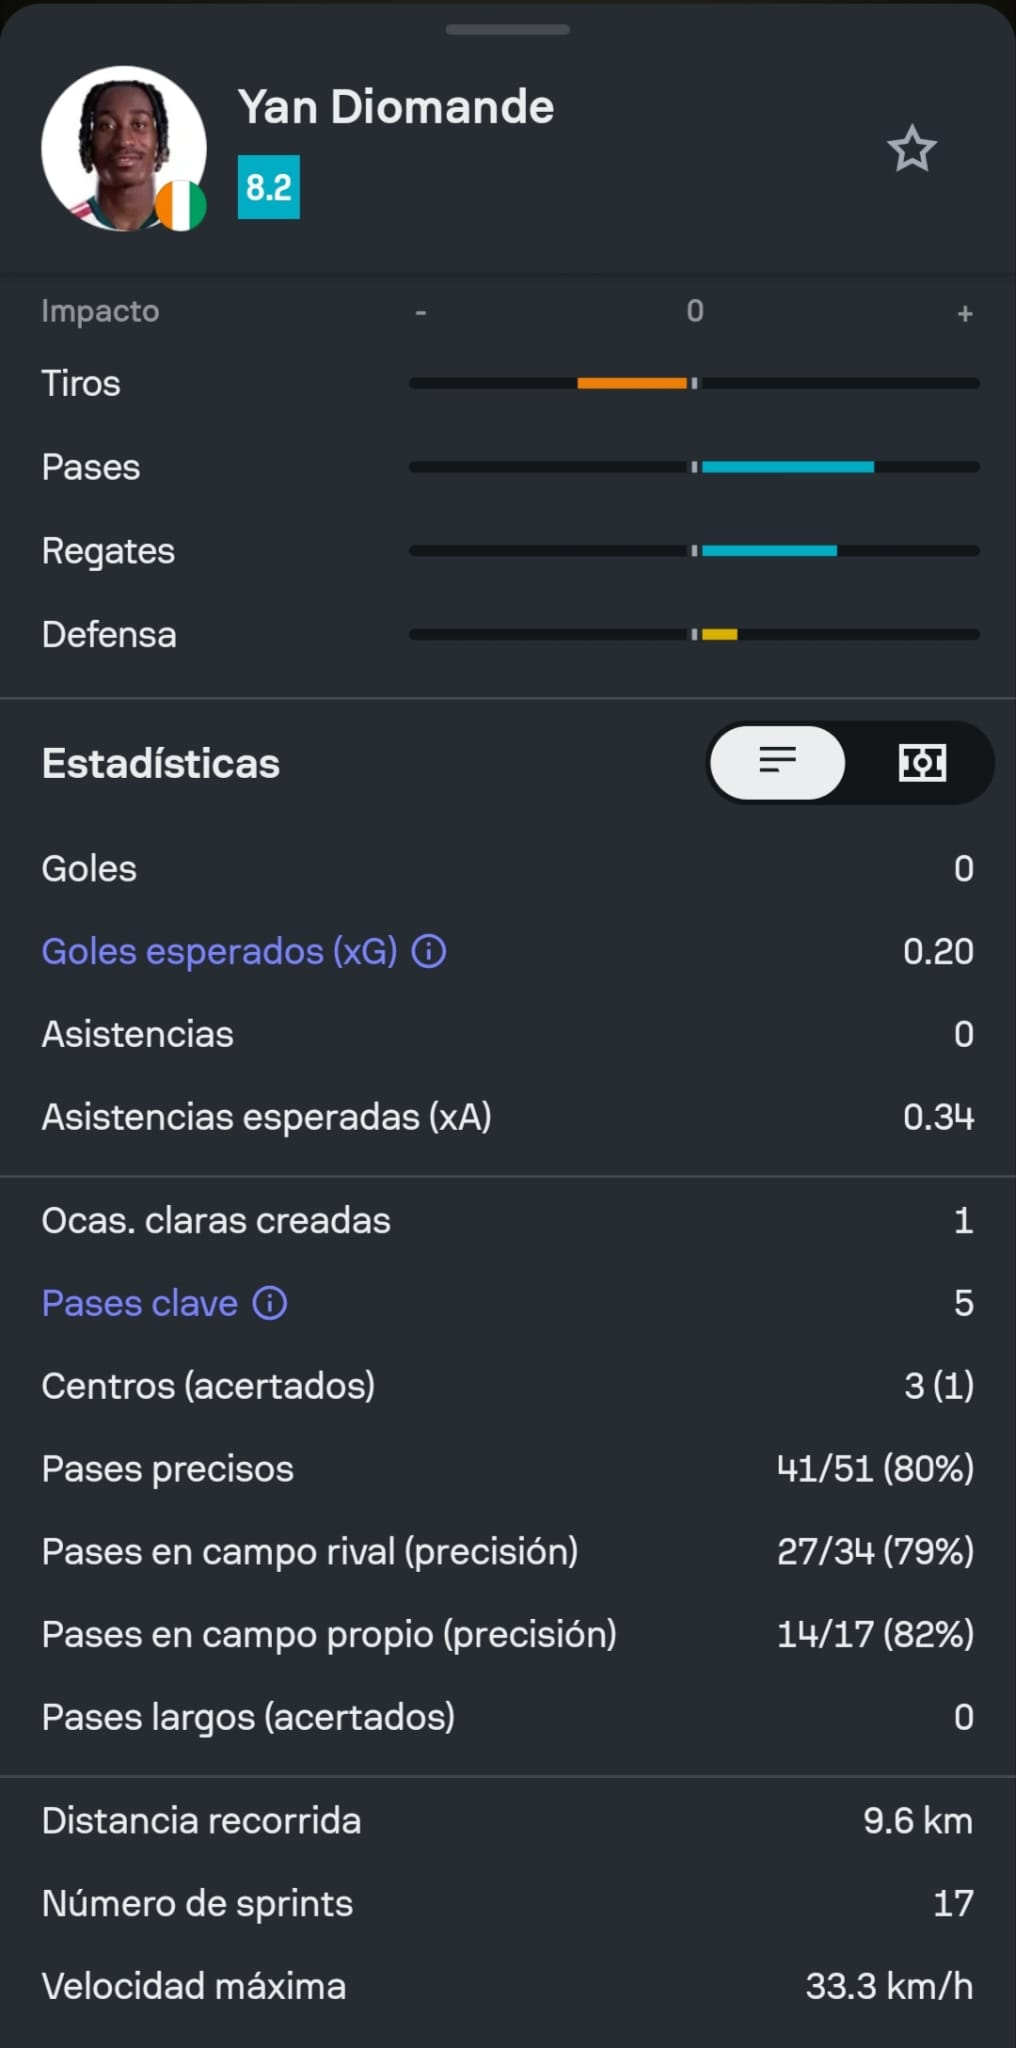
\includegraphics[width=0.5\linewidth]{figures/app_sofascore_stats.jpeg}
    \caption{Estadísticas mostradas}
    \label{fig:sofascore_stats}
  \end{subfigure}
  \hspace{0.5cm}
  \begin{subfigure}[b]{0.4\textwidth}
    \centering
    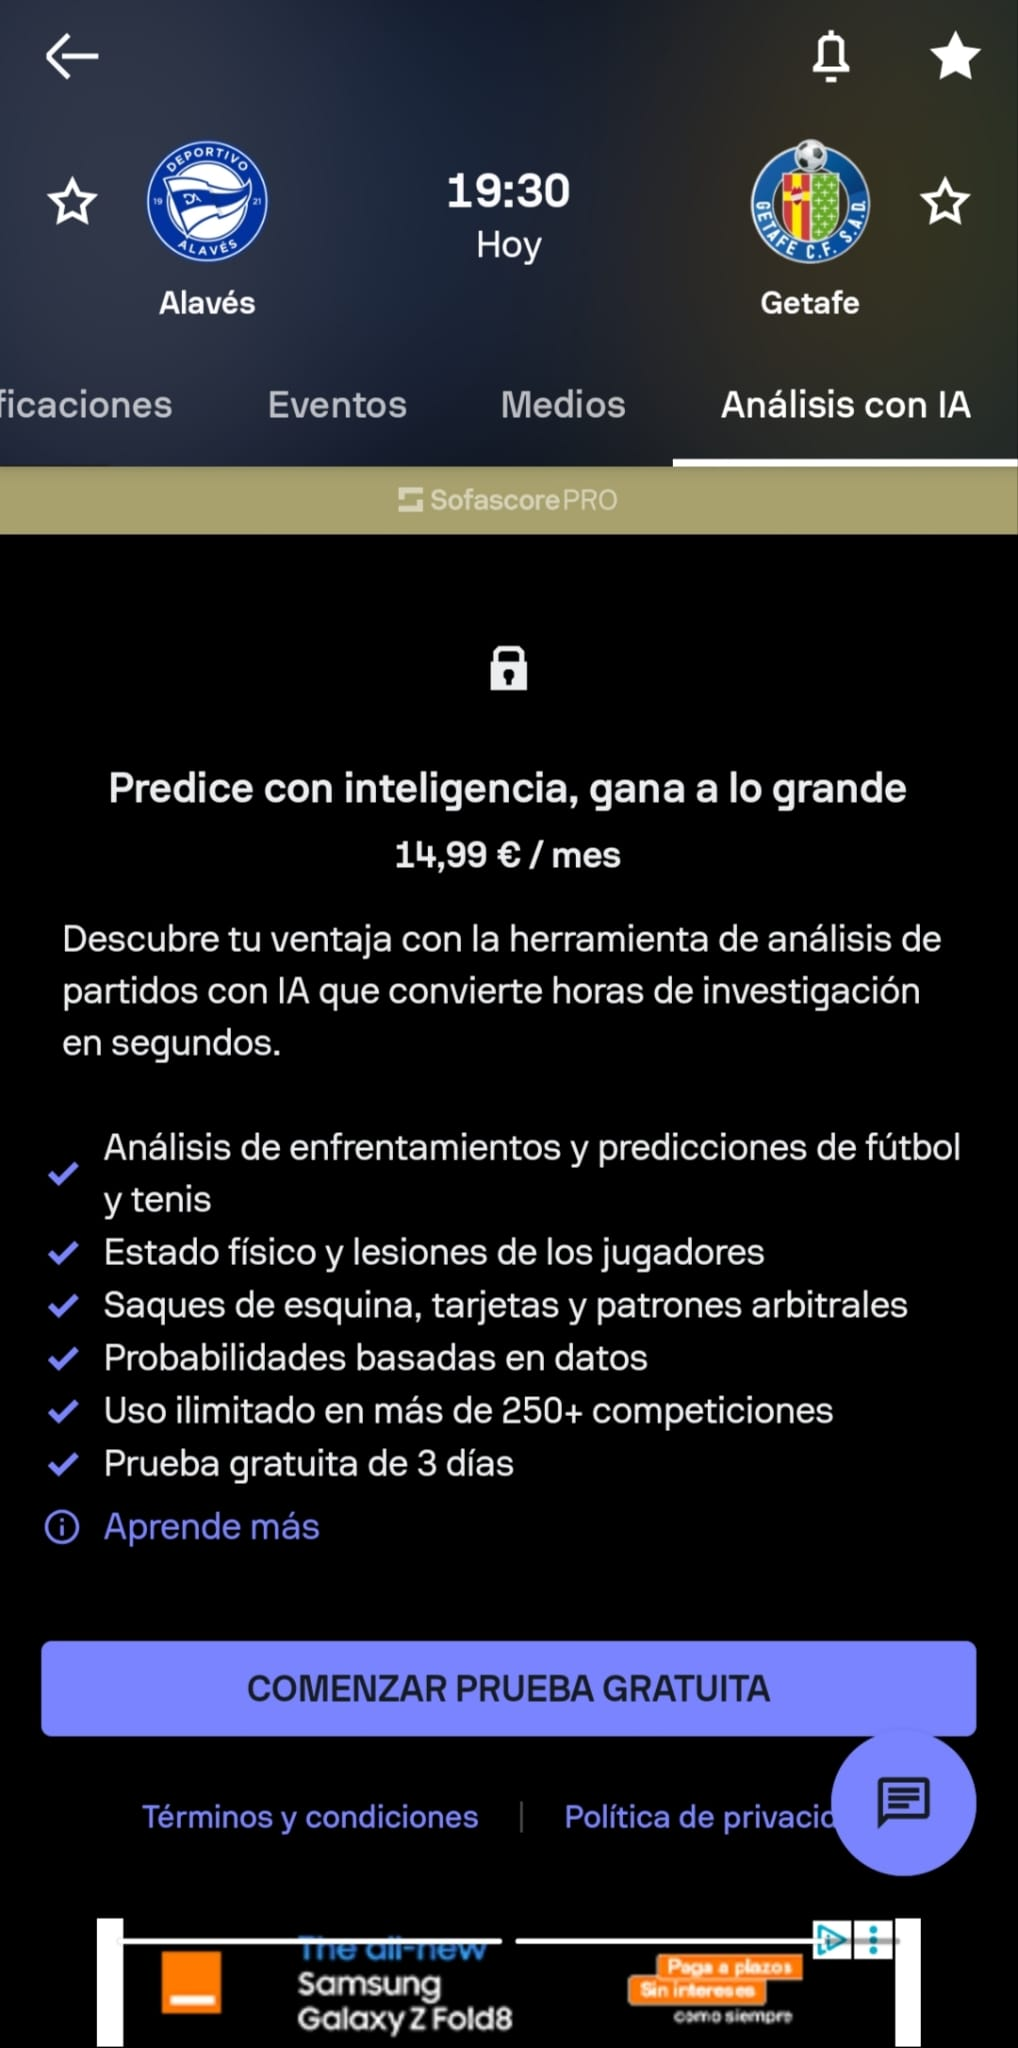
\includegraphics[width=0.5\linewidth]{figures/app_sofasocore_pago.jpeg}
    \caption{Funcionalidades de IA de pago}
    \label{fig:sofascore_ia}
  \end{subfigure}
  \caption{SofaScore}
  \label{fig:sofascore}
\end{figure}

\begin{table}[H]
\centering
\caption{Comparativa de funcionalidades entre aplicaciones de análisis de fútbol.}
\label{tab:comparativa_apps}
\renewcommand{\arraystretch}{1.2}

\begin{tabularx}{\textwidth}{|X|c|c|c|c|}
\hline
\textbf{Característica} & \textbf{BeSoccer} & \textbf{SofaScore} & \textbf{LaLiga} & \textbf{Propuesta} \\ \hline

Estadísticas históricas & \ding{51} & \ding{51} & \ding{51} & \ding{51} \\ \hline

Estadísticas avanzadas & Parcial & Sí & Parcial & \ding{51} \\ \hline

\textit{Dashboards} de \textit{business intelligence} & \ding{55} & \ding{55} & \ding{55} & \ding{51} \\ \hline

Análisis IA Gratis & \ding{51} & Básico & \ding{55} & \ding{51} \\ \hline

Predicción mediante IA & \ding{51} & Parcial & \ding{55} & \ding{51} \\ \hline

Simulación Monte Carlo & \ding{51} & \ding{55} & \ding{55} & \ding{51} \\ \hline

\textit{Clustering} de jugadores & \ding{55} & \ding{55} & \ding{55} & \ding{51} \\ \hline

Detección de necesidades de plantilla & \ding{55} & \ding{55} & \ding{55} & \ding{51} \\ \hline

Chatbot basado en IA & \ding{55} & \ding{55} & \ding{55} & \ding{51} \\ \hline

Simulación interactiva de temporada & \ding{55} & \ding{55} & \ding{55} & \ding{51} \\ \hline

Resultados en directo & \ding{51} & \ding{51} & \ding{51} & \ding{55} \\ \hline
\end{tabularx}
\end{table}

